\subsection{Convolutional Neural Network}
The following section will describe the TensorFlow Keras
\cite{tensorflow2015-whitepaper} model used in the prototype of the
Image Classification tool.  
After loading the images, the dataset was split into a training and
testing set, 80\% and 20\% respectively.

\subsection{Score Calculation}

    \subsubsection{Preference Gathering}
        This section will describe an example of the score calculation based
        on user criteria. Initially, the application asks the user certain
        preferences such as:
        \begin{enumerate}
            \item The trip budget
            \item Moderation of activities (How busy the trip needs to be)
            \item Users’ characteristics (based on Instagram Results)
            \item Number of people
            \item Where the user is going
            \item Date and time the user will be going
        \end{enumerate}

        \begin{figure}[H]
            \caption{The following figure includes some sample user preferences        }
            \centering
            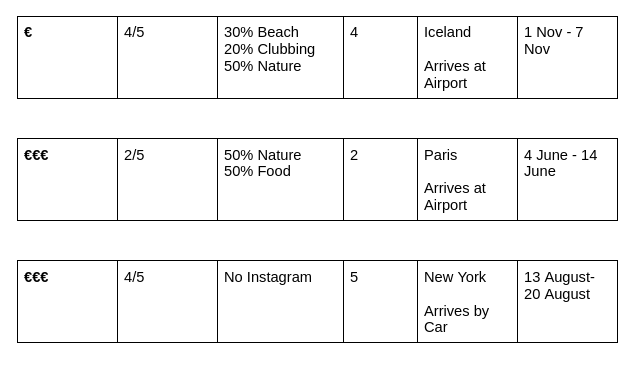
\includegraphics[scale=0.41]{SampleResults.png}
            \label{dataset}
        \end{figure}

        \subsection{Activity Details}
        Each Activity will contain its own details upon which a
        score is calculated. Some example of such parameters include:
        \begin{enumerate}
            \item Cost
            \item How close is the place to the user’s characteristics (from Instagram)
            \item At what time is the place open
            \item Approximately the amount of time people spend there (even based on user’s moderation)
            \item Place Importance
            \item What type of Weather is the place accessible
            \item Time to travel from the previous location
            \item Place reviews
            
        \end{enumerate}

        \begin{figure}[H]
            \caption{The following figure includes some sample activity details}
            \centering
            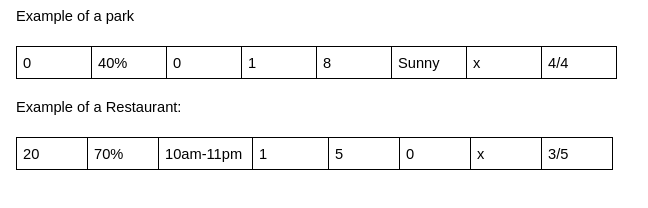
\includegraphics[scale=0.41]{SamplePlace.png}
            \label{dataset}
        \end{figure}

        \begin{figure}[H]
            \caption{The following figure includes some sample activity details}
            \centering
            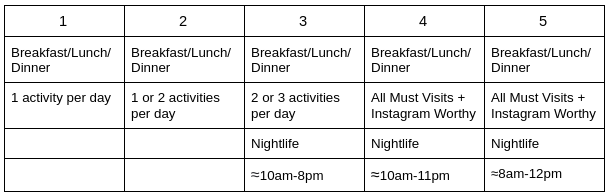
\includegraphics[scale=0.41]{UserModeration.png}
            \label{dataset}
        \end{figure}